\documentclass[11pt, oneside]{article}   	% use "amsart" instead of "article" for AMSLaTeX format
\usepackage{geometry}                		% See geometry.pdf to learn the layout options. There are lots.
\geometry{letterpaper}                   		% ... or a4paper or a5paper or ... 
%\geometry{landscape}                		% Activate for for rotated page geometry
%\usepackage[parfill]{parskip}    		% Activate to begin paragraphs with an empty line rather than an indent
\usepackage{graphicx}				% Use pdf, png, jpg, or eps� with pdflatex; use eps in DVI mode
								% TeX will automatically convert eps --> pdf in pdflatex		
\usepackage{amssymb}
\usepackage{amsmath}
\usepackage{parskip}
\usepackage{color}
\usepackage{hyperref}

\title{Newton's method}
%\author{The Author}
%\section{}
%\subsection*{}
\date{}							% Activate to display a given date or no date

\graphicspath{{/Users/telliott_admin/Dropbox/Tex/png/}}
% \begin{center} 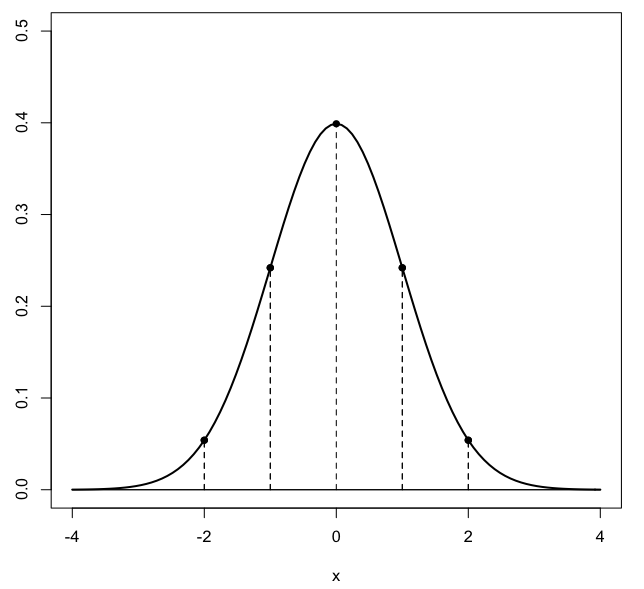
\includegraphics [scale=0.4] {gauss3.png} \end{center}
\begin{document}
\maketitle
\Large
Here is a method for finding roots of equations quickly, often called Newton's method, or the Newton-Raphson method.  As an example, here is a plot of the function
\[ f(x) = x^2 - 2 \]
\begin{center} 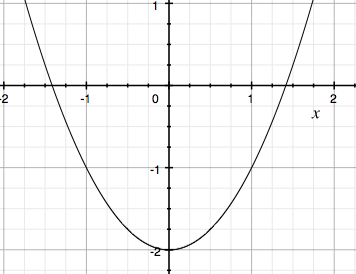
\includegraphics [scale=0.6] {sqrt2.png} \end{center}
which is equal to zero when $x = \pm \sqrt{2}$.  That is, we want the roots of the following equation
\[ x^2 - 2 = 0 \]
and more generally
\[ x^2 - N = 0 \]
to find the square root of some other number.  Pick a point $g$ (for guess).  It doesn't have to be a particularly good guess.  Then we need to construct the line tangent to the curve at that point, with slope $m=f'(g)$ and ask, where does this line intercept the $x$-axis?  The slope is $\Delta y/ \Delta x$.
\[ \frac{f(g) - 0}{g - g'} = f'(g) \]
$g'$ is the $x$-coordinate at the intercept.  Rearrange
\[ \frac{f(g)}{f'(g)} = g - g' \]
\[ g' = g - \frac{f(g)}{f'(g)} \]
\subsection*{square root problem}
For this particular problem, we have
\[ f(g) = g^2 - N \]
\[ f'(g) = 2g \]
\[ g' = g - \frac{g^2 - N}{2g} = \frac{1}{2} (g + \frac{N}{g}) \]
Which can be encapsulated into the following algorithm:
\begin{itemize}
\item Make a guess $g$ and compute $N/g$
\item Average $g$ and $N/g$ to find a new guess
\item Repeat until satisfied
\end{itemize}
The algorithm converges rapidly for most problems.

\tt{
2 \\
1.5 \\ 
1.41666666667 \\
1.41421568627 \\
1.41421356237 \\
1.41421356237
}

\end{document} 